\documentclass[11pt,]{article}
\usepackage{lmodern}
\usepackage{amssymb,amsmath}
\usepackage{ifxetex,ifluatex}
\usepackage{fixltx2e} % provides \textsubscript
\ifnum 0\ifxetex 1\fi\ifluatex 1\fi=0 % if pdftex
  \usepackage[T1]{fontenc}
  \usepackage[utf8]{inputenc}
\else % if luatex or xelatex
  \ifxetex
    \usepackage{mathspec}
  \else
    \usepackage{fontspec}
  \fi
  \defaultfontfeatures{Ligatures=TeX,Scale=MatchLowercase}
\fi
% use upquote if available, for straight quotes in verbatim environments
\IfFileExists{upquote.sty}{\usepackage{upquote}}{}
% use microtype if available
\IfFileExists{microtype.sty}{%
\usepackage{microtype}
\UseMicrotypeSet[protrusion]{basicmath} % disable protrusion for tt fonts
}{}
\usepackage[margin=1in]{geometry}
\usepackage{hyperref}
\hypersetup{unicode=true,
            pdftitle={Insecticide resistance evolution with mixtures and sequences : a model-based graphical introduction and summary},
            pdfauthor={Andy South and Ian Hastings},
            pdfborder={0 0 0},
            breaklinks=true}
\urlstyle{same}  % don't use monospace font for urls
\usepackage{longtable,booktabs}
\usepackage{graphicx,grffile}
\makeatletter
\def\maxwidth{\ifdim\Gin@nat@width>\linewidth\linewidth\else\Gin@nat@width\fi}
\def\maxheight{\ifdim\Gin@nat@height>\textheight\textheight\else\Gin@nat@height\fi}
\makeatother
% Scale images if necessary, so that they will not overflow the page
% margins by default, and it is still possible to overwrite the defaults
% using explicit options in \includegraphics[width, height, ...]{}
\setkeys{Gin}{width=\maxwidth,height=\maxheight,keepaspectratio}
\IfFileExists{parskip.sty}{%
\usepackage{parskip}
}{% else
\setlength{\parindent}{0pt}
\setlength{\parskip}{6pt plus 2pt minus 1pt}
}
\setlength{\emergencystretch}{3em}  % prevent overfull lines
\providecommand{\tightlist}{%
  \setlength{\itemsep}{0pt}\setlength{\parskip}{0pt}}
\setcounter{secnumdepth}{0}
% Redefines (sub)paragraphs to behave more like sections
\ifx\paragraph\undefined\else
\let\oldparagraph\paragraph
\renewcommand{\paragraph}[1]{\oldparagraph{#1}\mbox{}}
\fi
\ifx\subparagraph\undefined\else
\let\oldsubparagraph\subparagraph
\renewcommand{\subparagraph}[1]{\oldsubparagraph{#1}\mbox{}}
\fi

%%% Use protect on footnotes to avoid problems with footnotes in titles
\let\rmarkdownfootnote\footnote%
\def\footnote{\protect\rmarkdownfootnote}

%%% Change title format to be more compact
\usepackage{titling}

% Create subtitle command for use in maketitle
\newcommand{\subtitle}[1]{
  \posttitle{
    \begin{center}\large#1\end{center}
    }
}

\setlength{\droptitle}{-2em}
  \title{Insecticide resistance evolution with mixtures and sequences : a
model-based graphical introduction and summary}
  \pretitle{\vspace{\droptitle}\centering\huge}
  \posttitle{\par}
  \author{Andy South and Ian Hastings}
  \preauthor{\centering\large\emph}
  \postauthor{\par}
  \predate{\centering\large\emph}
  \postdate{\par}
  \date{2017-04-11}

\usepackage{setspace}
\doublespacing
\usepackage{lineno}
\linenumbers

\begin{document}
\maketitle

\subsubsection{version 12}\label{version-12}

\subsubsection{alternative titles:}\label{alternative-titles}

\subsubsection{Evolution of insecticide resistance with insecticide
mixtures and sequences : an accessible model to promote
understanding.}\label{evolution-of-insecticide-resistance-with-insecticide-mixtures-and-sequences-an-accessible-model-to-promote-understanding.}

\subsubsection{An accessible model to promote understanding of the
evolution of insecticide resistance : insecticide effectiveness
predicted to be key to the relative performance of
mixtures.}\label{an-accessible-model-to-promote-understanding-of-the-evolution-of-insecticide-resistance-insecticide-effectiveness-predicted-to-be-key-to-the-relative-performance-of-mixtures.}

\subsubsection{A tutorial, primer \ldots{}}\label{a-tutorial-primer}

\subsubsection{Insecticide effectiveness predicted to be most important
factor determining whether insecticide mixtures can slow evolution of
resistance.}\label{insecticide-effectiveness-predicted-to-be-most-important-factor-determining-whether-insecticide-mixtures-can-slow-evolution-of-resistance.}

Target : Malaria journal (other suggestions welcome)

THIS IS A CONFIDENTIAL COPY OF THE MS. Please do not circulate without
the permission of one of the authors. Comments and suggestions welcome

\subsection{Abstract}\label{abstract}

\emph{must be 350 words, currently 351}

\subparagraph{Background}\label{background}

Insecticide resistance threatens the control of vectors and particularly
malaria. New insecticides are being developed to address this. Potential
strategies for using new insecticides include mixtures, sequences and
rotations and there are recommendations for how best to implement these
to manage resistance. There is, however, limited recent, accessible
modelling work addressing the evolution of resistance under different
operational strategies. Previous work concludes that preferred
strategies will be situation specific. There is potential to improve the
level of mechanistic understanding within the operational community of
how insecticide resistance can be expected to evolve in response to
different strategies.

This paper develops an accessible, mechanistic picture of how the
evolution of insecticide resistance is likely to respond to potential
intervention strategies to help guide both management and policy. The
aim is to reach an audience unlikely to read a more detailed modelling
paper. We use our model to develop a mechanistic understanding of how
insecticide resistance is expected to increase with the use of
insecticides in isolation, sequence and mixtures. The model flexibly
represents two independent genes coding for resistance to two
insecticides. We look principally at the ability of the insecticides to
kill susceptible mosquitoes, how much resistance counteracts this, the
proportion of mosquitoes that are exposed to insecticides and costs of
resistance.

\subparagraph{Results}\label{results}

We use the model to demonstrate the evolution of resistance under
different inputs and how this fits with intuitive reasoning about the
selection pressure exerted by insecticides. We show that an insecticide
used in a mixture, relative to alone, always prompts slower evolution of
resistance, but resistance to the two insecticides may evolve more
slowly when used in sequence. We show that the ability of insecticides
to kill susceptible mosquitoes (effectiveness), has the most influence
on whether resistance to two insecticides is likely to arise faster in a
mixture or sequence.

\subparagraph{Conclusions}\label{conclusions}

Our model makes more open the process of insecticide resistance
evolution and how it is likely to respond to insecticide use. We provide
a simple user-interface allowing further exploration
(\url{https://andysouth.shinyapps.io/MixSeqResist1}). These tools can
contribute to operational decisions in insecticide resistance
management.

\subsection{Keywords}\label{keywords}

insecticide resistance; public health; mosquitoes; vector-borne
diseases; infectious diseases; malaria; population genetics

\subsection{Background}\label{background-1}

Insecticide resistance is a problem for malaria {[}1{]}{[}2{]}{[}3{]}
other vector borne diseases {[}4{]} and agriculture {[}5{]}. Malaria
alone still results in hundreds of thousands of deaths per year. Recent
malaria control efforts have centred on treated bed nets and indoor
residual spraying, both reliant on insecticides. Treated nets were
recently estimated to contribute 68\% and indoor residual spraying 13\%
to averting more than 500 million falciparum malaria cases between 2000
and 2015 {[}6{]}. A recent malaria transmission model {[}7{]} predicts
that even low pyrethroid resistance is likely to increase malaria
incidence in Africa by reducing the performance of bed nets.

The WHO produced a Global Plan for Insecticide Resistance Management in
malaria vectors (GPIRM){[}1{]} which includes recommendations on
operational strategies for managing resistance including the use of
insecticide mixtures when they become available. Efforts are under way
to develop new insecticides that will be effective in the light of
existing resistance and allow additional options within insecticide
resistance management. The Innovative Vector Control Consortium (IVCC)
was set up in 2005 to develop new vector control tools and particularly
new insecticides to address insecticide resistance in malaria
transmitting mosquitoes {[}8{]}{[}9{]}. Three new insecticides are now
in development {[}9{]} and likely to be available around 2020 {[}2{]}.
It is important that decisions about how best to use the new
insecticides to delay the onset of resistance are made before
insecticides are released {[}3{]}.

Modelling studies have investigated the evolution of insecticide
resistance in insecticide mixtures including in a public health context
e.g. {[}10{]}{[}11{]}{[}12{]} but much of the work was done more than 20
years ago and there remained some confusion about the results {[}13{]}.
In an earlier paper {[}13{]} we described the technical details of a
flexible model used to investigate the relative benefits of mixtures and
sequences. Here we provide an accessible summary of the model and use
selected parameter values to describe mechanistically how the evolution
of resistance is influenced by different inputs. This mechanistic
understanding can contribute to the debate on the relative merits of
different insecticide strategies extending existing frameworks
{[}12{]}{[}4{]}{[}5{]}{[}1{]}.

Our modelling approach focuses on the change in frequency of a single
resistance gene for each insecticide. It is likely that genes conferring
resistance are present in populations even prior to exposure to novel
insecticides thus leading to the potential for selection {[}14{]}.

\subsection{Methods}\label{methods}

The simulation represents a population of randomly mixing individuals
using standard population genetic approaches to avoid the need to follow
every individual. One gene or locus is represented for each insecticide.
Each individual has two copies of the gene and there are two potential
alleles per locus. Each allele confers either resistance or
susceptibility to the insecticide. Thus individuals can either have both
resistance genes (RR homozygous), both susceptible genes (SS) or one of
each (SR, heterozygous). The combination of the two genes is termed the
genotype. Fitness is the main currency of the model, representing how
much each genotype survives and reproduces. The fitness of the SS
genotype in absence of the insecticide is set at a maximum value of 1.
All other fitnesses are less, determined by alleles, exposure to the
insecticide and other inputs that can be set in the model. These inputs
include the effectiveness of the insecticide, the dominance of the
resistance allele and the ability of resistance to restore fitness in
the presence of the insecticide (see Table 1).

\textbf{Table 1. Parameters inflencing the development of insecticide
resistance}

\begin{longtable}[]{@{}ll@{}}
\toprule
\begin{minipage}[b]{0.28\columnwidth}\raggedright\strut
Parameter\strut
\end{minipage} & \begin{minipage}[b]{0.66\columnwidth}\raggedright\strut
Description\strut
\end{minipage}\tabularnewline
\midrule
\endhead
\begin{minipage}[t]{0.28\columnwidth}\raggedright\strut
1. Effectiveness\strut
\end{minipage} & \begin{minipage}[t]{0.66\columnwidth}\raggedright\strut
proportion of susceptible (SS) insects killed by exposure to
insecticide\strut
\end{minipage}\tabularnewline
\begin{minipage}[t]{0.28\columnwidth}\raggedright\strut
2. Exposure\strut
\end{minipage} & \begin{minipage}[t]{0.66\columnwidth}\raggedright\strut
proportion of insects exposed to insecticide\strut
\end{minipage}\tabularnewline
\begin{minipage}[t]{0.28\columnwidth}\raggedright\strut
3. Resistance restoration\strut
\end{minipage} & \begin{minipage}[t]{0.66\columnwidth}\raggedright\strut
ability of resistance (RR) to restore fitness of insects exposed to
insecticide\strut
\end{minipage}\tabularnewline
\begin{minipage}[t]{0.28\columnwidth}\raggedright\strut
4. Dominance of restoration\strut
\end{minipage} & \begin{minipage}[t]{0.66\columnwidth}\raggedright\strut
sets fitness of heterozygous (SR) insects between that of SS \& RR in
presence of insecticide\strut
\end{minipage}\tabularnewline
\begin{minipage}[t]{0.28\columnwidth}\raggedright\strut
5. Frequency\strut
\end{minipage} & \begin{minipage}[t]{0.66\columnwidth}\raggedright\strut
frequency of resistance alleles within the population\strut
\end{minipage}\tabularnewline
\begin{minipage}[t]{0.28\columnwidth}\raggedright\strut
6. Cost of resistance\strut
\end{minipage} & \begin{minipage}[t]{0.66\columnwidth}\raggedright\strut
fitness of resistant (RR) insects in absence of insecticide\strut
\end{minipage}\tabularnewline
\begin{minipage}[t]{0.28\columnwidth}\raggedright\strut
7. Dominance of cost\strut
\end{minipage} & \begin{minipage}[t]{0.66\columnwidth}\raggedright\strut
sets fitness of heterozygous (SR) insects between that of SS \& RR in
absence of insecticide\strut
\end{minipage}\tabularnewline
\bottomrule
\end{longtable}

The calculation of fitness for each genotype when considering just a
single insecticide is illustrated in Figure 1. In the model itself this
is repeated for both insecticides and the fitnesses multiplied. Firstly
the exposure input determines the proportion of the population in the
left and right panels (exposed and not exposed). For those that are
exposed (left panel) insecticide effectiveness sets the fitness for SS
and resistance restoration `restores' a portion of the fitness for RR. A
value of 1 for resistance restoration would bring the fitness of RR back
to 1 (equivalent to the unexposed SS), a value of 0 for resistance
restoration would lead to the RR having the same fitness as SS in the
presence of the insecticide and effectively there would be no
resistance. We use `Resistance restoration' to represent how much the RR
genotype restores fitness in the presence of the insecticide. The
`selection coefficient' of resistance, that may be seen referred to
elsewhere {[}10{]}, can be calculated by multiplying resistance
restoration by insecticide effectiveness. Cost of resistance determines
the fitness of RR in the portion of the population not exposed to the
insecticide.

Dominance of restoration determines how the fitness for SR sits between
that of SS and RR for those that are exposed to the insecticide. For
those that are not exposed, fitness of SS is set to 1 by definition and
resistance cost determines the fitness of RR. Dominance of cost
determines how the fitness for SR sits between that of SS and RR in the
absence of the insecticide (Figure 1).

The simulation proceeds through generations. In each generation
selection is represented by multiplying genotype frequencies in the
population by their relative fitness. This acts to make the fitter
alleles more common over time. Separate sexes and standard sexual
reproduction with recombination is included. There is also the potential
to set exposure rates to be different for males and females to represent
their different behaviours but we do not explore that here.

So far this description just considers a single insecticide and
associated resistance allele. In the model itself a second insecticide
and resistance allele are included and overall fitness is calculated by
multiplying the two results. This allows the model to represent
populations exposed to two insecticides together in a mixture.

The model outputs the change in resistance allele frequencies over time
measured in generations. We extract the number of generations at which a
resistance allele frequency of 50\% is reached and term this
`time-to-resistance'. Using a 50\% threshold is consistent with previous
modelling analyses e.g. {[}10{]}{[}15{]}. Preliminary investigations
showed that using other potential thresholds of 25 or 75\% gave very
similar results.

We investigate three insecticide use strategies.

\begin{enumerate}
\def\labelenumi{\arabic{enumi}.}
\tightlist
\item
  single insecticide
\item
  two insecticides used in sequence, replacing the first with a second
  once the frequency of resistance alleles reaches a threshold of 50\%
\item
  two insecticides used in a mixture (concurrently)
\end{enumerate}

The model is implemented in R {[}16{]}, the code is hosted on Github
{[}17{]} and we provide an on-line user interface {[}18{]} (Fig 2)
enabling the reader to change inputs and run the model themselves.

\subsection{Results}\label{results-1}

\subsubsection{Single insecticide}\label{single-insecticide}

For single insecticide use, higher values of insecticide effectiveness,
exposure, resistance restoration and its dominance all resulted in
faster resistance spread (Fig 3 A-D) and thus fewer generations to reach
a resistance threshold of 0.5. This makes intuitive sense as all
increase the impact of the insecticide and thus increase selection for
resistance. Similarly, higher values of starting resistance frequency
also resulted in shorter times to resistance thresholds (Fig 4A) through
the even simpler mechanism that less change is required to reach the
threshold.

Cost of resistance (Fig 4B) and its dominance (not shown) had the
opposite effect. Higher values led to a slower development of
resistance. Again this is intuitive because costs reduce the advantage
of resistance and decrease selection. These effects of inputs on single
insecticide use are summarised in Table 2.

\subsubsection{Two insecticides}\label{two-insecticides}

When two insecticides are used we can compare the relative performance
of a mixture with sequential use. Each panel in Figures 5-9 compares
mixture and sequence for a single combination of inputs. To help
understand the mechanisms influencing this relative performance we start
with a single base scenario and demonstrate changing inputs
individually. In this base scenario we set effectiveness, exposure,
resistance restoration, and dominance at 0.5, the starting frequencies
of resistance to 0.01 and cost of resistance to 0. Resistance arises
slower for sequential than mixture for this base scenario (Fig 5A).
Resistance to both insecticides in the mixture follow the same path and
reach the threshold at the same time (as would be expected given that
they have identical input parameters). When used in sequence the curve
(dashed) for each insecticide individually is steeper than in the
mixture but, because they happen one after the other, it takes longer
for both to reach the resistance threshold (Fig 5A). Thus the
time-to-resistance for the mixture divided by the sequence is less than
1 at 0.8.

\paragraph{Insecticide exposure and
effectiveness}\label{insecticide-exposure-and-effectiveness}

Increasing exposure (the proportion of insects that come into contact
with the insecticides) (Fig 5C) decreases the time-to-resistance for
both the sequential and mixture strategy. The effect on the mixture is
greater so time-to-resistance remains longer for the sequence (the ratio
decreasing from 0.8 to 0.6). In contrast keeping the exposure constant
and increasing effectiveness (the proportion of SS insects that are
killed by contact) of one of the insecticides (Fig 5B) results in a
longer time-to-resistance for the mixture relative to the sequence (and
the ratio increasing from 0.8 to 1.2). The longer time-to-resistance for
the mixture results from a slower increase in resistance for the less
effective insecticide. Resistance to the less effective insecticide in
the mixture increases slowly initially and then speeds up after the more
effective insecticide has reached the resistance threshold. This points
a mechanism whereby the more effective insecticide initially slows the
rate of evolution of resistance to the less effective one.

The results is that a more effective insecticide increases
time-to-resistance when used in a mixture (compare the solid lines in
Fig 5A \& B). This is opposite to what happens when used in sequence
(compare the red dashed line in Fig 5A \& B) and in isolation (Fig 2A),
when more effective insecticides shortened times-to-resistance.

In summary increasing effectiveness can favour mixtures moving from
column 1 to 2 in Figure 5, and increasing exposure can favour sequences
moving from row 1 to 2 in Figure 5. Reduced male exposure with respect
to female, as might be expected for male mosquitoes not seeking blood
meals, had a similar effect to changing overall exposure. Reducing male
exposure (not shown) increased times-to-resistance and favoured mixtures
over sequences.

Increasing the effectiveness further of either or both insecticides
increases the performance of mixtures over sequences in terms of
time-to-resistance. Figure 6A uses the same inputs as Fig 5B. From this
scenario a higher effectiveness for insecticide2 (Fig 6C) or insecticide
1 (Fig 6B) or both (Fig 6D) all result in a greater positive difference
in time-to-resistance for mixture over sequence. This again points to
how more effective insecticides can slow resistance to another when used
in a mixture.

\paragraph{Resistance restoration and
dominance}\label{resistance-restoration-and-dominance}

Increasing resistance restoration or its dominance decreases
time-to-resistance for both sequences and mixtures (Fig 7) in the same
way that it did for sole use (Fig 3). The result is that increasing
either or both of dominance and resistance restoration (Figs 7B,C,D)
doesn't change the relative time-to-resistance for mixtures and
sequences from that in the base scenario (Fig 7A) where it takes
resistance longer to develop for the sequence. So, unlike effectiveness
and exposure, the levels of resistance restoration and dominance do not
effect whether a mixture or a sequence are likely to be favoured.

\paragraph{Starting frequencies of
resistance}\label{starting-frequencies-of-resistance}

Changing the starting frequency of resistance had a similar effect on
time to resistance for both sequences and mixtures and thus had little
effect on their relative performance. For example taking the base
scenario and reducing the starting frequency of one resistance allele
did not change from sequence being favoured (compare Fig 8C to 8A).
Similarly taking a scenario in which time-to-resistance is longer for a
mixture (Fig 8B) and decreasing the starting frequency of that
resistance allele did not change the fact that the mixture was favoured
(Fig 8D).

\paragraph{Costs of resistance}\label{costs-of-resistance}

Increasing the cost of resistance to one insecticide in a mixture leads
resistance to that insecticide to evolve more slowly (compare the solid
red line to the solid blue line in Figure 9C, the red line is for the
resistance with the higher cost). The resistance with the higher cost
also increases more slowly in the mixture relative to when it is used in
sequence (compare the solid red line to the dotted red line in Fig 9C).
The greater effect of cost on mixtures means the advantage of sequences
over mixtures in Fig 9A (and Fig 5A) is removed in Fig 9C. With costs
set to 0 time-to-resistance for mixture divided by sequence is 0.8 in
Fig 9A and 1 in Fig 9C. At higher insecticide effectiveness the benefit
of mixture over sequence is improved as seen by comparing Fig 9D to 9B.

A summary of the effects of inputs on the evolution of resistance for
mixtures is given in Table 3 and for the difference between mixtures and
sequences in Table 4. The mechanisms identified in the tables are
covered further in the discussion.

\paragraph{Linkage disequilibrium}\label{linkage-disequilibrium}

It has previously been suggested {[}10{]}{[}1{]} that using an
insecticide to which there was existing resistance in a mixture with a
new insecticide with little resistance could lead to more rapid
evolution of resistance to the latter through a process termed linkage
disequilibrium. Figure 8 C\&D show how our model predicts that linkage
disequilibrium does not lead to more rapid evolution of resistance to
the newer insecticide. In Figures 8 C\&D the newer insecticide with
lower starting resistance (in red) leads to faster resistance when used
alone (red dotted) than when used in a mixture (red solid).

\subsection{Discussion}\label{discussion}

Resistance responds to insecticide use in the model in ways that we can
explain mechanistically through the process of selection. This
mechanistic explanation can help us develop a more robust understanding
of how we would expect resistance to evolve in the field.

When single insecticide use was investigated (Figs 3-4) higher values of
inputs that increased the selective advantage of resistance all led to
more rapid evolution resistance, and higher values for cost led to
slower evolution of (Fig 4B).

These mechanisms, explaining the response of resistance to single
insecticide use under different input values, are summarised in Table 2.
Referring to figure 1 can help explain these. Exposure and effectiveness
act by decreasing the fitness of all genotypes, dominance of restoration
acts by increasing fitness of SR and resistance-restoration acts by
increasing fitness of RR \& SR. Cost acts by decreasing the fitness of
RR and SR for those not exposed.

\paragraph{Two insecticides}\label{two-insecticides-1}

Using two insecticides either in sequence or in mixtures differs from
the use of a single insecticide and, where it differs can again help us
to understand the dynamics of resistance evolution. Our base scenario
(Fig 5A) shows curves for resistance to both insecticides in the mixture
that are shallower than those for sequential use. The shallower curves
for the mixture can be explained by each insecticide killing individuals
that are resistant to the other insecticide. Thus each insecticide
reduces the selection pressure for the increase in resistance to the
other and could be said to `protect' the other. However this protection
is not necessarily enough to ensure that resistance arises more slowly
in a mixture relative to a sequential strategy. Resistance can evolve
more slowly for both insecticides in sequential use, despite being
faster for each, because they occur one after the other. In Figure 5A it
takes 60 generations for resistance to reach the threshold for each
insecticide in the sequence, and 90 when they are applied together in
the mixture, so the sequence is still favoured because 2x60 is greater
than 90. Incraesing the effectiveness of on insecticide to Fig 5B
decreases the added times for the sequence to 90 and increases those for
the mixture to 115 thus changing the order and favouring the mixture.

The mechanism for this change can be sen by comparing the shape of the
curves in Figs 5A \& B. In the mixture, resistance to insecticide 1
(with the increased effectiveness) rises at a similar speed in both
figures. However, the increased effectiveness of insecticide 1 causes
resistance to insecticide 2 to increase more slowly initially in the
mixture. Once insecticide 1 reaches resistance of around 50\% at around
50 generations, the curve for insecticide 2 becomes steeper. Once the
first insecticide has become ineffective due to resistance it stops
killing individuals that are resistant to the second insecticide, loses
its protective effect and thus stops slowing the rise in resistance to
the second insecticide. A similar effect is visible when the
effectiveness of both insecticides are increased (Fig 6C). The identical
resistance curves for each insecticide in the mixture are shallower than
at the lower effectiveness (Fig 5A) because more individuals resistant
to each insecticide are being killed by the other insecticide. In this
case the `protection' given to both insecticides by the other declines
at the same rate so we don't see the change in slope seen in Fig 5B.

Fig 5B also demonstrates that when two insecticides have a different
effectiveness in a mixture, other parameters being equal, resistance
will be expected to increase faster to the more effective insecticide.
The more effective insecticide prompts both a) higher selection pressure
for it's own resistance and b) greater `protection' reducing the rise in
resistance to the other insecticide.

\paragraph{Difference between exposure and
effectiveness}\label{difference-between-exposure-and-effectiveness}

It seems initially counter-intuitive that whereas increasing
effectiveness slows the development of resistance for mixtures,
increasing exposure speeds it up. Increasing the exposure to both
insecticides results in a decrease in time-to-resistance (from 90
generations in Fig 5A to 40 generations in Fig 5C) where increasing the
effectiveness of both insecticides by the same amount results in a
slight increase (from 90 in Fig 5A to 115 in Fig 5B). This contrasts
with the identical effects that exposure and effectiveness have on a
single insecticide (Figs 3 A,B) and on insecticides in sequence (the red
dashed lines are the same in Figs 5B \& 5C). This difference, that
exposure reduces times-to-resistance for a mixture and effectiveness
increases it, was unexpected for us.

\paragraph{Costs of resistance}\label{costs-of-resistance-1}

Costs of resistance favour mixtures in these analyses because the
evolution of resistance is slowed more by cost in a mixture than in a
sequence (compare the red solid lines for a mixture to the red dotted
line for a sequence in Fig 9C and D). It seems that the protective
effect of the other insecticide in a mixture interacts with the cost of
resistance to reduce selection pressure more than in a sequence.

The effects of cost of resistance become more as the frequency of
resistance increases. The resistance curves for two insecticides in a
mixture that differ only in their cost of resistance, diverge more as
the frequency of resistance increases (Fig 9C). This makes intuitive
sense, as the frequency of resistance genes increases the impact of
fitness costs associated with those genes becomes greater. Thus
differences due to cost are less noticeable at low resistance
frequencies and become more noticeable at higher resistance frequencies.
Thus if a lower resistance threshold was used cost would have less of an
effect and if a higher resistance threshold was used cost would have
more of an effect. Also note that if the costs are set even higher than
we set them here (e.g.~above 0.2) they can maintain resistance
frequencies below 1 or lead to their decline. Unfortunately, we do not
expect such high costs to occur in operational settings.

Relatedly, when there are costs of resistance, the frequency of
resistance for insecticides that are not being used is likely to
decline. Thus the frequency of resistance for the first insecticide in a
sequence, after it has been replaced, may decline to a level where it
becomes operationally useful again. As such a repeated sequential
strategy could offer benefits over mixtures not considered here. To
incorporat this one would need to use a more detailed metric than
time-to-resistance.

\paragraph{Caveats}\label{caveats}

Our model examines solely the evolution of resistance and not the
control of mosquitoes or malaria. Different insecticide use strategies,
as well as effecting the evolution of resistance, will also influence
both the numbers of vectors and their propensity to transmit the disease
{[}19{]}. Insecticide resistance could reduce vector transmission of
disease (e.g.~by reduced lifespan of the vector) or increase
transmission (e.g.~by reduced immunity of the vector to the disease)
{[}19{]}. Our model would predict that the best strategy for limiting
the development of resistance in the short term would be to use no
insecticide. Of course, using no insecticide could have serious
consequences for mosquito and malaria abundance. The challenge is to
develop good strategies for delivering mosquito and malaria control in
the short term while sustaining their operational capacity in the longer
term by restricting the development of resistance. Others are combining
models of population genetics and population dynamics to investigate
these trade-offs {[}20{]}.

In our model we represented insecticide interaction as being additive
within the mixture. This is consistent with recent work on aphids
{[}21{]}, although that work did also indicate some synergistic effects.
Our model has the potential to incorporate either synergistic or
antagonistic effects too.

The development of insecticide resistance in operational field settings
is subject to considerable uncertainty {[}2{]}. The model we present
here is able to cover the range of that uncertainty, yet in this paper,
to develop an understanding of the key mechanisms we restrict our
explorations to a limited region of parameter space (e.g.~holding most
inputs constant at intermediate values while modifying single inputs in
isolation). Thus there is the potential that the system may behave
differently in the field than we describe here. However, the results
presented here are supported by an earlier analysis where we ran 10,000
unique scenarios varying more inputs {[}13{]}. This previous analysis
also highlighted the relative importance of insecticide effectiveness
and exposure in determining the relative performance of mixtures and
sequences. In addition we provide an on-line user interface to the model
{[}18{]} and enabling readers to investigate model behaviour in areas of
parameter space we have not shown.

\paragraph{Consistency with previous
work}\label{consistency-with-previous-work}

The predicted responses of resistance presented here can be put into the
context of previous work and recommendations. Earlier modelling work has
made sometimes contrasting predictions and these can be explained by the
details of their structure and input choices. One model predicted that
``the use of mixtures is always more effective in delaying the onset of
resistance often by many orders of magnitude''{[}11{]}. That model
assumed that SS genotypes were always killed, RR always survived, and
that a constant 10\% of mosquitoes escaped the insecticide. This would
be represented in our model by a very high `insecticide effectiveness'
of 1, a `resistance restoration' of 1 and an `exposure' of 0.9. This
result is consistent with our prediction that the very high
effectiveness is likely to favour mixtures over sequences (e.g.~see Fig
6D and Table 4).

A subsequent model {[}22{]} lead to the following more pessimistic
conclusion about the potential of mixtures : ``As a result of incomplete
coverage and residue decay, the mortality of susceptible homozygotes is
rarely consistently high enough for pesticide mixtures to be effective''
{[}22{]}. This ``mortality of susceptible homozygotes'' is equivalent to
our insecticide effectiveness. Again this points to the importance of
effectiveness and the question of whether the effectiveness levels
needed to make mixtures better are attainable operationally. Our result
showing that decreasing exposure favours mixtures over sequences is also
consistent with figure 3 from that paper {[}22{]}.

One consistent aspect of the results presented here can seem to
contradict published advice and has been questioned when we have
presented model results. Our model predicts that lower insecticide
effectiveness or exposure will lead to slower spread of resistance in
sole use and sequences (Figs 3 \& 5, Table 2). This is consistent with
expectations that lower effectiveness and exposure would lead to lower
mortality of susceptibles and thus lower selection pressure for
resistance {[}22{]}. This can seem to contradict recommendations that
poor implementation of insecticide interventions can promote the
development of resistance. e.g.~from {[}5{]} ``Certain pest control
practices have consistently been shown to exacerbate the loss of
susceptible pest populations and the development of resistance. These
include: \ldots{} - the use of application rates that are below or above
those recommended on the label, - poor coverage of the area being
treated \ldots{}''.

Poor implementation would likely cause lower effectiveness of and
exposure to insecticides, so how can this increase the potential for
resistance when our model suggests it would be decreased ? The
explanation for this apparent difference is in the effect of dominance.
Poor application can reduce the mortality of heterozygotes (RS) thus
effectively increasing the dominance of the resistant allele and
increasing its rate of evolution {[}23{]}{[}5{]}. Our model results are
consistent with this, showing that increasing dominance of restoration
leads to faster spread of resistance (Fig 3C, 7). So, the effect of poor
implementation of an insecticide intervention on resistance could be
either positive or negative depending on the relative effects on
dominance of the resistance gene, insecticide effectiveness and
exposure. Similarly, the effects of poor application on the relative
benefits of mixtures and sequences will depend on these trade-offs
because of our result that effectivenes favours mixtures, exposure
favours sequences and higher dominance favours neither (Table 4).

\paragraph{Implications}\label{implications}

Experience from agriculture where single interventions have been
associated with a rapid development of resistance have led for calls for
a more Integrated Vector Management composed of a series of partially
effective tools {[}24{]}. It is suggested that such an integrated
approach is more sustainable and `evolution-proof' {[}24{]}. A similar
combining of interventions has been advocated to cover mosquitoes
exhibiting different behaviours {[}25{]}. Mosquitoes with different
behaviours e.g.~feeding outdoors and/or on animals are likely to result
in lower exposures to insecticides in nets or sprayed on walls. This
lower exposure could favour mixtures over sequences as we have
indicated. In both cases our modelling approach could be used to
investigate implications for the development of resistance.

\emph{TODO bits to incorporate into discussion :}

\emph{todo more reference to {[}12{]} who made many of these points 25
years ago}

\emph{Insecticides with some repellency will reduce exposure to the
insecticide and thus, as shown here, are likely to slow the evolution of
resistance and favour mictures over sequences. This would need to be
balanced with a likely loss in protection to the population as a whole
provided by the insecticide {[}15{]}.}

\emph{This model can explore when a mixture strategy may be favoured
over a sequence purely for the evolution of resistance. Other factors
also need to be considered. On the positive side a mixture is likely to
kill more vectors and may also limit their ability to transmit the
disease. On the negative side a mixture is more expensive.}

\emph{todo, somewhere earlier say good thing about effectiveness \&
exposure is that they can be modified}

\paragraph{Conclusions}\label{conclusions-1}

We have developed flexible, modern model that can replicate previous
modelling work and outputs that help us understand the mechanisms by
which different insecticide application strategies may be favoured. For
assessing the relative benefits of mixtures and sequences we have
demonstrated the likely importance of insecticide effectiveness and
exposure and costs of resistance. High insecticide effectiveness favours
mixtures through the protective effect of one insecticide on the other.
High exposure favours sequences because of the higher selection
pressures on both resistances together in a mixture. High costs of
resistance can favour mixtures because the selection pressures on both
resistances are reduced. Similar processes will occur in other
strategies such as rotations and mosaics and we are starting to
investigate them. Predictions from the model can be tested against data
from trials of new insectides to help advance guidelines on good
practice.

\subsubsection{Declarations}\label{declarations}

TODO see
\url{https://malariajournal.biomedcentral.com/submission-guidelines/preparing-your-manuscript/research-article}

\subparagraph{Ethics approval and consent to
participate}\label{ethics-approval-and-consent-to-participate}

Not applicable

\subparagraph{Consent for publication}\label{consent-for-publication}

Not applicable

\subparagraph{Availability of data and
material}\label{availability-of-data-and-material}

\subparagraph{Competing interests}\label{competing-interests}

\subparagraph{Funding}\label{funding}

\subparagraph{Authors' contributions}\label{authors-contributions}

AS conceived the paper, re-factored the model code, performed the
analyses and wrote the first and subsequent versions of the paper. IH
conceived the modelling approach, developed the first version of the
model in collaboration with Bethany Levick, explained concepts to AS and
reviewed and commented on all manuscript versions.

\subparagraph{Acknowledgements}\label{acknowledgements}

Thank you to Bethany Levick who developed the first version of the model
code.

\pagebreak

\textbf{Table 2. Effect of inputs on resistance when insecticides used
singly or in sequence}

\begin{longtable}[]{@{}lll@{}}
\toprule
\begin{minipage}[b]{0.28\columnwidth}\raggedright\strut
Parameter to increase\strut
\end{minipage} & \begin{minipage}[b]{0.10\columnwidth}\raggedright\strut
effect on resistance evolution\strut
\end{minipage} & \begin{minipage}[b]{0.53\columnwidth}\raggedright\strut
Mechanism\strut
\end{minipage}\tabularnewline
\midrule
\endhead
\begin{minipage}[t]{0.28\columnwidth}\raggedright\strut
1. Effectiveness\strut
\end{minipage} & \begin{minipage}[t]{0.10\columnwidth}\raggedright\strut
faster\strut
\end{minipage} & \begin{minipage}[t]{0.53\columnwidth}\raggedright\strut
reduced fitness of SS in presence of insecticide\strut
\end{minipage}\tabularnewline
\begin{minipage}[t]{0.28\columnwidth}\raggedright\strut
2. Exposure\strut
\end{minipage} & \begin{minipage}[t]{0.10\columnwidth}\raggedright\strut
faster\strut
\end{minipage} & \begin{minipage}[t]{0.53\columnwidth}\raggedright\strut
reduced fitness of SS overall\strut
\end{minipage}\tabularnewline
\begin{minipage}[t]{0.28\columnwidth}\raggedright\strut
3. Dominance of restoration\strut
\end{minipage} & \begin{minipage}[t]{0.10\columnwidth}\raggedright\strut
faster\strut
\end{minipage} & \begin{minipage}[t]{0.53\columnwidth}\raggedright\strut
increased fitness of SR in presence of insecticide\strut
\end{minipage}\tabularnewline
\begin{minipage}[t]{0.28\columnwidth}\raggedright\strut
4. Resistance restoration\strut
\end{minipage} & \begin{minipage}[t]{0.10\columnwidth}\raggedright\strut
faster\strut
\end{minipage} & \begin{minipage}[t]{0.53\columnwidth}\raggedright\strut
increased fitness of RR in presence of insecticide\strut
\end{minipage}\tabularnewline
\begin{minipage}[t]{0.28\columnwidth}\raggedright\strut
5. Frequency\strut
\end{minipage} & \begin{minipage}[t]{0.10\columnwidth}\raggedright\strut
faster\strut
\end{minipage} & \begin{minipage}[t]{0.53\columnwidth}\raggedright\strut
less change needed to reach resistance threshold\strut
\end{minipage}\tabularnewline
\begin{minipage}[t]{0.28\columnwidth}\raggedright\strut
6. Cost of resistance\strut
\end{minipage} & \begin{minipage}[t]{0.10\columnwidth}\raggedright\strut
slower\strut
\end{minipage} & \begin{minipage}[t]{0.53\columnwidth}\raggedright\strut
reduced fitness of RR in absence of insecticide\strut
\end{minipage}\tabularnewline
\bottomrule
\end{longtable}

\textbf{Table 3. Effect of inputs on resistance when insecticides used
in a mixture}

\begin{longtable}[]{@{}lll@{}}
\toprule
\begin{minipage}[b]{0.27\columnwidth}\raggedright\strut
Parameter to increase\strut
\end{minipage} & \begin{minipage}[b]{0.12\columnwidth}\raggedright\strut
effect on resistance evolution\strut
\end{minipage} & \begin{minipage}[b]{0.52\columnwidth}\raggedright\strut
Mechanism\strut
\end{minipage}\tabularnewline
\midrule
\endhead
\begin{minipage}[t]{0.27\columnwidth}\raggedright\strut
1. Effectiveness\strut
\end{minipage} & \begin{minipage}[t]{0.12\columnwidth}\raggedright\strut
\textbf{slower}\strut
\end{minipage} & \begin{minipage}[t]{0.52\columnwidth}\raggedright\strut
one insecticide reduces the fitness of individuals resistant to the
other thereby reducing selection pressure from the other\strut
\end{minipage}\tabularnewline
\begin{minipage}[t]{0.27\columnwidth}\raggedright\strut
2. Exposure\strut
\end{minipage} & \begin{minipage}[t]{0.12\columnwidth}\raggedright\strut
faster (but less than for single)\strut
\end{minipage} & \begin{minipage}[t]{0.52\columnwidth}\raggedright\strut
reduced fitness of individuals susceptible to one insecticide increases
selection pressure for that resistance. However at the same time
selection pressure is reduced by reduced fitness of resistant
individuals caused by the other insecticide\strut
\end{minipage}\tabularnewline
\begin{minipage}[t]{0.27\columnwidth}\raggedright\strut
3. Dominance of restoration\strut
\end{minipage} & \begin{minipage}[t]{0.12\columnwidth}\raggedright\strut
faster\strut
\end{minipage} & \begin{minipage}[t]{0.52\columnwidth}\raggedright\strut
increased fitness of heterozygotes\strut
\end{minipage}\tabularnewline
\begin{minipage}[t]{0.27\columnwidth}\raggedright\strut
4. Resistance restoration\strut
\end{minipage} & \begin{minipage}[t]{0.12\columnwidth}\raggedright\strut
faster\strut
\end{minipage} & \begin{minipage}[t]{0.52\columnwidth}\raggedright\strut
increased fitness of resistants\strut
\end{minipage}\tabularnewline
\begin{minipage}[t]{0.27\columnwidth}\raggedright\strut
5. Frequency\strut
\end{minipage} & \begin{minipage}[t]{0.12\columnwidth}\raggedright\strut
faster\strut
\end{minipage} & \begin{minipage}[t]{0.52\columnwidth}\raggedright\strut
less change needed to reach resistance threshold\strut
\end{minipage}\tabularnewline
\begin{minipage}[t]{0.27\columnwidth}\raggedright\strut
6. Cost of resistance\strut
\end{minipage} & \begin{minipage}[t]{0.12\columnwidth}\raggedright\strut
slower\strut
\end{minipage} & \begin{minipage}[t]{0.52\columnwidth}\raggedright\strut
reduced fitness of resistants in absence of insecticide\strut
\end{minipage}\tabularnewline
\bottomrule
\end{longtable}

\pagebreak

\textbf{Table 4. Effect of inputs on the difference between mixture and
sequential use}

\begin{longtable}[]{@{}lll@{}}
\toprule
\begin{minipage}[b]{0.28\columnwidth}\raggedright\strut
Parameter to increase\strut
\end{minipage} & \begin{minipage}[b]{0.10\columnwidth}\raggedright\strut
increase favours mix or sequence\strut
\end{minipage} & \begin{minipage}[b]{0.53\columnwidth}\raggedright\strut
Mechanism\strut
\end{minipage}\tabularnewline
\midrule
\endhead
\begin{minipage}[t]{0.28\columnwidth}\raggedright\strut
1. Effectiveness\strut
\end{minipage} & \begin{minipage}[t]{0.10\columnwidth}\raggedright\strut
mixture\strut
\end{minipage} & \begin{minipage}[t]{0.53\columnwidth}\raggedright\strut
Higher effectiveness gives faster resistance for sequence and slower
resistance in mixture\strut
\end{minipage}\tabularnewline
\begin{minipage}[t]{0.28\columnwidth}\raggedright\strut
2. Exposure\strut
\end{minipage} & \begin{minipage}[t]{0.10\columnwidth}\raggedright\strut
sequence\strut
\end{minipage} & \begin{minipage}[t]{0.53\columnwidth}\raggedright\strut
Higher exposure gives faster resistance for sequence and mixture but the
greater effect on mixture favours sequence.\strut
\end{minipage}\tabularnewline
\begin{minipage}[t]{0.28\columnwidth}\raggedright\strut
3. Dominance of restoration\strut
\end{minipage} & \begin{minipage}[t]{0.10\columnwidth}\raggedright\strut
neither\strut
\end{minipage} & \begin{minipage}[t]{0.53\columnwidth}\raggedright\strut
Higher dominance gives faster resistance in both sequences and mixtures
such that the difference between them is not changed.\strut
\end{minipage}\tabularnewline
\begin{minipage}[t]{0.28\columnwidth}\raggedright\strut
4. Resistance restoration\strut
\end{minipage} & \begin{minipage}[t]{0.10\columnwidth}\raggedright\strut
neither\strut
\end{minipage} & \begin{minipage}[t]{0.53\columnwidth}\raggedright\strut
As for dominance of restoration. Higher resistance restoration gives
faster resistance in both sequences and mixtures such that the
difference between them is not changed.\strut
\end{minipage}\tabularnewline
\begin{minipage}[t]{0.28\columnwidth}\raggedright\strut
5. Frequency\strut
\end{minipage} & \begin{minipage}[t]{0.10\columnwidth}\raggedright\strut
neither\strut
\end{minipage} & \begin{minipage}[t]{0.53\columnwidth}\raggedright\strut
As for dominance and resistance restoration. Higher starting frequencies
give faster resistance in both sequences and mixtures such that the
difference between them is not changed.\strut
\end{minipage}\tabularnewline
\begin{minipage}[t]{0.28\columnwidth}\raggedright\strut
6. Cost of resistance\strut
\end{minipage} & \begin{minipage}[t]{0.10\columnwidth}\raggedright\strut
mixture\strut
\end{minipage} & \begin{minipage}[t]{0.53\columnwidth}\raggedright\strut
Higher costs slow the evolution of resistance more in a mixture than
when used in sequence (but with higher costs in a sequence there is a
greater chance for resistance levels to decline for the insecticide not
being used).\strut
\end{minipage}\tabularnewline
\bottomrule
\end{longtable}

\pagebreak

\subsection{Figures}\label{figures}

\begin{figure}

\includegraphics{paper2_resistance_mechanisms_mixtures_files/figure-latex/Fig1-1} \hfill{}

\caption{The effect of model inputs on the fitness of genotypes for a single insecticide. Fitness is shown on the y-axis and the different genotypes (SS, SR, RR) on the x axis. Firstly the exposure input determines the proportion of the population in the left and right panels (exposed and not exposed). For those that are exposed (left panel) insecticide effectiveness sets the fitness for SS, resistance restoration 'restores' a portion of the fitness for RR and dominance of restoration determines how the fitness for SR lies between that of SS and RR. For those that are not exposed, fitness of SS is set to 1 by definition, resistance cost determines the fitness of RR and again dominance of cost determines how the fitness for SR sits between that of SS and RR. In this example effectiveness=0.8, dominance of restoration=0.6, resistance restoration=0.5, dominance of cost=0.6 and resistance cost=0.3.}\label{fig:Fig1}
\end{figure}

\begin{figure}[htbp]
\centering
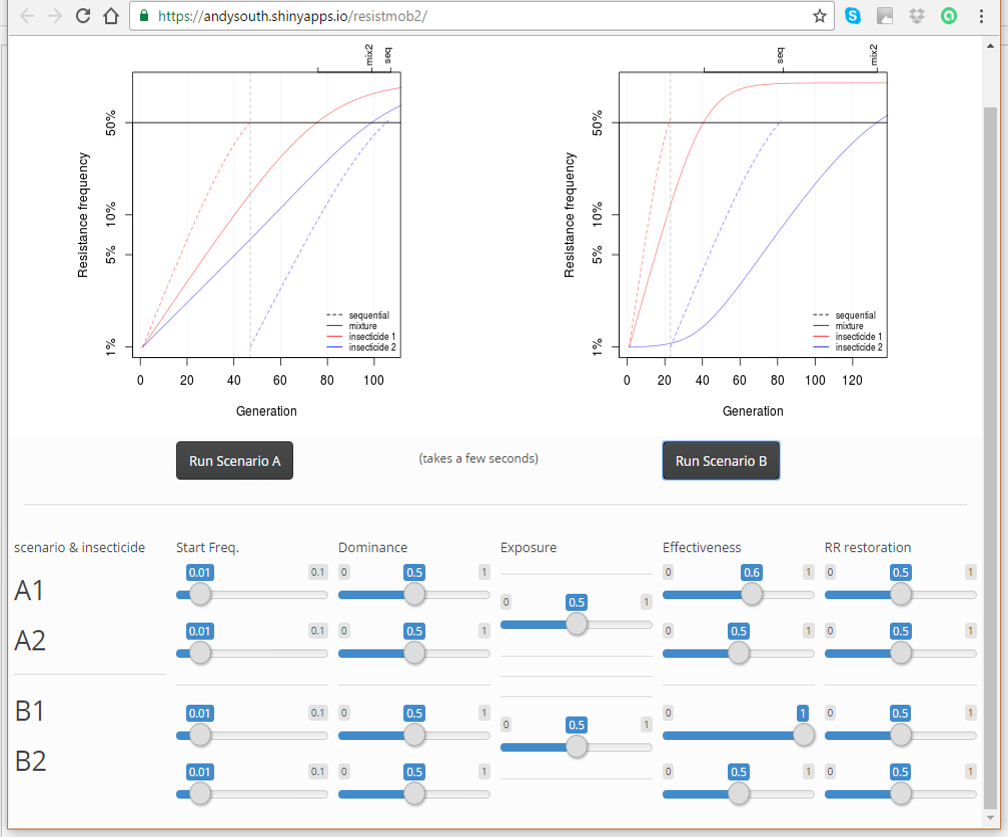
\includegraphics{paper2_UI1.png}
\caption{Screenshot of one online model user interface, accessible at :
\url{https://andysouth.shinyapps.io/resistmob2/}. The user can modify
values of the input parameters considered in this paper using simple
sliders and run the model to get graphs of resulting resistance
frequency over time. Two scenarios (A and B) can be run and the results
viewed side by side. This makes it easy to explore the effect of
changing individual inputs.}
\end{figure}

\begin{figure}

\includegraphics{paper2_resistance_mechanisms_mixtures_files/figure-latex/Fig3-1} \hfill{}

\caption{Single insecticide use and the effect of inputs on changing resistance frequency over time. A. Effectiveness, B. Exposure, C. Dominance of restoration, D. Resistance restoration. Increasing any of the inputs (going from red to blue) results in shorter times-to-resistance. For each panel the chosen input was varied in isolation with the remaining inputs set to 0.5, except for starting frequency of resistance which was set to 0.01). }\label{fig:Fig3}
\end{figure}

\begin{figure}

\includegraphics{paper2_resistance_mechanisms_mixtures_files/figure-latex/Fig4-1} \hfill{}

\caption{Single insecticide use and the effect of inputs on changing resistance frequency over time. A. Starting frequency, B. Cost of resistance. Increasing the starting frequency decreases the number of generations taken to reach resistance thresholds. Increasing costs of resistance increases time-to-resistance.}\label{fig:Fig4}
\end{figure}

\begin{figure}

\includegraphics{paper2_resistance_mechanisms_mixtures_files/figure-latex/Fig5-1} \hfill{}

\caption{Influence of insecticide effectiveness and exposure on time-to-resistance for mixtures and sequences. Exposure to the insecticides is increased from row 1 (A and B) to row 2 (C and D). The effectiveness of one insecticide is increased from column 1 (A and C) to column2 (B and D). On the upper X axis 's' and 'm' indicate where the 50 percent resistance threshold is reached for the sequence and the mixture. In the lower right of each panel the the ratio of time-to-resistance for mixture/sequence is shown rounded to 1 decimal place to give an indication of the relative performance of mixtures and sequences.  A. All control inputs equal at 0.5 : time-to-resistance is longer for sequential use, B. Effectiveness of insecticide1 increased from 0.5 to 0.8 : time-to-resistance is longer for the mixture, C. Exposure increased to 0.8 : time-to-resistance is longer for sequential use, D. Effectiveness of insecticide1 and exposure increased to 0.8 : time-to-resistance equal for mixture and sequence. Increasing effectiveness increases times-to-resistance for mixtures and improves their performance relative to sequences. Increasing exposure decreases times-to-resistance for mixtures and reduces their performance relative to sequences. }\label{fig:Fig5}
\end{figure}

\begin{figure}

\includegraphics{paper2_resistance_mechanisms_mixtures_files/figure-latex/Fig6-1} \hfill{}

\caption{Influence of the effectiveness of both insecticides on time-to-resistance for mixtures and sequences. Effectiveness of insecticide 2 is increased from row 1 (A and B) to row 2 (C and D). The effectiveness of insecticide 1 is increased from column 1 (A and C) to column2 (B and D). The 's' and 'm' on the upper X axis and 'mix/seq' in the lower right of each panel stand for sequence and mixture and are explained in the legend to Fig 5. A. Effectiveness of insecticide1 increased from 0.5 to 0.8, B. Effectiveness of insecticide1 increased from 0.5 to 1, C. Effectiveness of insecticides 1 and 2 increased to 0.8, D. Effectiveness of insecticide2 0.8 and of insecticide1 1. With the effectiveness of at least one insecticide greater than or equal to 0.8, times-to-resistance are longer for the mixture in all scenarios.}\label{fig:Fig6}
\end{figure}

\begin{figure}

\includegraphics{paper2_resistance_mechanisms_mixtures_files/figure-latex/Fig7-1} \hfill{}

\caption{Influence of dominance and resistance restoration on time-to-resistance for mixtures and sequences. Dominance of the allele coding for resistance to insecticide 1 is increased from row 1 (A and B) to row 2 (C and D). Resistance restoration for the allele coding for resistance to insecticide 1 is increased from column 1 (A and C) to column2 (B and D). The 's' and 'm' on the upper X axis and mix/seq in the lower right of each panel stand for sequence and mixture and are explained in the legend to Fig 5. A. All control inputs equal at 0.5, B. Resistance restoration for insecticide1 increased from 0.5 to 0.8, C. Dominance for insecticide1 increased to 0.8, D. Resistance restoration and dominance for insecticide1 increased to 0.8. Changing dominance and resistance restoration does not change the relative ordering of mixtures and sequences, time-to-resistance remains longest for sequences in all 4 scenarios.}\label{fig:Fig7}
\end{figure}

\begin{figure}

\includegraphics{paper2_resistance_mechanisms_mixtures_files/figure-latex/Fig8-1} \hfill{}

\caption{Influence of starting frequencies of resistance on time-to-resistance for mixtures and sequences. Starting frequency of the gene conferring resistance to insecticide 1 is decreased from row 1 (A and B) to row 2 (C and D). Effectiveness of insecticide 1 is increased from column 1 (A and C) to column2 (B and D). The 's' and 'm' on the upper X axis and mix/seq in the lower right of each panel stand for sequence and mixture and are explained in the legend to Fig 5. A. All control inputs equal at 0.5, starting frequencies of resistance at 0.01, B. Effectiveness for insecticide1 increased from 0.5 to 0.8, C. Starting frequency of resistance for insecticide1 decreased from 0.01 to 0.001, D. Effectiveness for insecticide1 increased from 0.5 to 0.8 and starting frequency for insecticide1 decreased from 0.01 to 0.001. In these scenarios the starting frequencies do not change better performance of sequences at low effectiveness and mixtures at high effectiveness.}\label{fig:Fig8}
\end{figure}

\begin{figure}

\includegraphics{paper2_resistance_mechanisms_mixtures_files/figure-latex/Fig 9 cost of 1 resistance-1} \hfill{}

\caption{Influence of cost of resistance on time-to-resistance for mixtures and sequences. Row 1 (A and B) same as Fig. 5 with no cost of resistance, row 2 (C and D) cost of resistance set to 0.15 with dominance of cost set to 0.5. The 's' and 'm' on the upper X axis and mix/seq in the lower right of each panel stand for sequence and mixture and are explained in the legend to Fig 5. The increase in cost of resistance from A. to C. removes the advantage of sequence relative to mixture. The ratio of time-to-resistance for the mixture divided by that for the sequence goes from 0. to 1. Costs seem to favour mixtures in these plots. Also be aware that costs would lead to a decline in the frequency of resistance for the first insecticide in a sequence when it stops being used.}\label{fig:Fig 9 cost of 1 resistance}
\end{figure}

\pagebreak

\subsection{References}\label{references}

\hypertarget{refs}{}
\hypertarget{ref-WHO2012}{}
1. WHO: \emph{Global plan for insecticide resistance management in
malaria vectors (GPIRM).} Geneva. 2012:130.

\hypertarget{ref-Ranson2016}{}
2. Ranson H, Lissenden N: \textbf{Insecticide Resistance in African
Anopheles Mosquitoes: A Worsening Situation that Needs Urgent Action to
Maintain Malaria Control}. \emph{Trends in Parasitology} 2016,
\textbf{32}:187--196.

\hypertarget{ref-Hemingway2016}{}
3. Hemingway J, Ranson H, Magill A, Kolaczinski J, Fornadel C, Gimnig J,
Coetzee M, Simard F, Roch DK, Hinzoumbe CK, Pickett J, Schellenberg D,
Gething P, Hoppé M, Hamon N: \textbf{Averting a malaria disaster: Will
insecticide resistance derail malaria control?} \emph{The Lancet} 2016,
\textbf{387}:1785--1788.

\hypertarget{ref-IRAC2011}{}
4. IRAC: \emph{Prevention and Management of Insecticide Resistance in
Vectors of Public Health Importance}. 2011:71.

\hypertarget{ref-FAO2012}{}
5. FAO: \emph{Guidelines on Prevention and Management of Pesticide
Resistance}. Rome; 2012:55.

\hypertarget{ref-Bhatt2015}{}
6. Bhatt S, Weiss DJ, Cameron E, Bisanzio D, Mappin B, Dalrymple U,
Battle KE, Moyes CL, Henry A, Eckhoff PA, Wenger EA, Briët O, Penny MA,
Smith TA, Bennett A, Yukich J, Eisele TP, Griffin JT, Fergus CA, Lynch
M, Lindgren F, Cohen JM, Murray CLJ, Smith DL, Hay SI, Cibulskis RE,
Gething PW: \textbf{The effect of malaria control on Plasmodium
falciparum in Africa between 2000 and 2015.} \emph{Nature} 2015,
\textbf{526}:207--11.

\hypertarget{ref-Churcher2016}{}
7. Churcher TS, Lissenden N, Griffin JT, Worrall E, Ranson H:
\textbf{The impact of pyrethroid resistance on the efficacy and
effectiveness of bednets for malaria control in Africa}. \emph{eLife}
2016, \textbf{5}:e16090.

\hypertarget{ref-Hemingway2006}{}
8. Hemingway J, Beaty BJ, Rowland M, Scott TW, Sharp BL: \textbf{The
Innovative Vector Control Consortium: improved control of mosquito-borne
diseases}. \emph{Trends in Parasitology} 2006, \textbf{22}:308--312.

\hypertarget{ref-IVCC2016}{}
9. IVCC: \textbf{Annual Report 2015-16}. 2016.

\hypertarget{ref-Curtis1985}{}
10. Curtis CF: \textbf{Theoretical models of the use of insecticide
mixtures for the management of resistance}. \emph{Bulletin of
Entomological Research} 1985, \textbf{75}:259.

\hypertarget{ref-Mani1985}{}
11. Mani GS: \textbf{Evolution of resistance in the presence of two
insecticides.} \emph{Genetics} 1985, \textbf{109}:761--783.

\hypertarget{ref-Roush1989}{}
12. Roush RT: \textbf{Designing resistance management programs: How can
you choose?} \emph{Pesticide Science} 1989, \textbf{26}:423--441.

\hypertarget{ref-Levick2017}{}
13. Levick B, South A, Hastings IM: \textbf{A Two-locus Model of The
Evolution of Insecticide Resistance to Inform and Optimise Public Health
Insecticide Deployment Strategies.} \emph{PLOS Computational Biology}
2017.

\hypertarget{ref-Liu2015}{}
14. Liu N: \textbf{Insecticide Resistance in Mosquitoes: Impact,
Mechanisms, and Research Directions}. \emph{Annual Review of Entomology}
2015, \textbf{60}:537--559.

\hypertarget{ref-Birget2015}{}
15. Birget PLG, Koella JC: \textbf{A genetic model of the effects of
insecticide-treated bed nets on the evolution of
insecticide-resistance}. \emph{Evolution, medicine, and public health}
2015, \textbf{2015}:205--215.

\hypertarget{ref-RCoreTeam2016}{}
16. R Core Team: \textbf{R: A language and environment for statistical
computing.} 2016.

\hypertarget{ref-South2017}{}
17. South A: \textbf{https://github.com/AndySouth/resistance}.

\hypertarget{ref-South2017a}{}
18. South A: \textbf{Online model user interface :
https://andysouth.shinyapps.io/resistmob2/}. 2017.

\hypertarget{ref-Rivero2010}{}
19. Rivero A, Vézilier J, Weill M, Read AF, Gandon S:
\textbf{Insecticide control of vector-borne diseases: When is
insecticide resistance a problem?} \emph{PLoS Pathogens} 2010.

\hypertarget{ref-Barbosa2017}{}
20. Barbosa S, Kay K, Chitnis N, Hastings IM, Tropical S:
\textbf{Modelling the public health impact of insecticide deployment on
malaria-transmitting mosquito populations and its role in driving
insecticide resistance .} 2017:1--58.

\hypertarget{ref-Taillebois2016}{}
21. Taillebois E, Thany SH: \textbf{The differential effect of low-dose
mixtures of four pesticides on the pea aphid Acyrthosiphon pisum}.
\emph{Insects} 2016, \textbf{7}:1--7.

\hypertarget{ref-Roush1998}{}
22. Roush RT: \textbf{Two-toxin strategies for management of
insecticidal transgenic crops: can pyramiding succeed where pesticide
mixtures have not?} \emph{Philosophical Transactions of the Royal
Society B: Biological Sciences} 1998, \textbf{353}:1777--1786.

\hypertarget{ref-Barbosa2011}{}
23. Barbosa S, Black IV WC, Hastings I: \textbf{Challenges in estimating
insecticide selection pressures from mosquito field data}. \emph{PLoS
Neglected Tropical Diseases} 2011, \textbf{5}.

\hypertarget{ref-Thomas2012}{}
24. Thomas MB, Godfray HCJ, Read AF, Berg H van den, Tabashnik BE,
Lenteren JC van, Waage JK, Takken W: \textbf{Lessons from agriculture
for the sustainable management of Malaria vectors}. \emph{PLoS Medicine}
2012, \textbf{9}:7--10.

\hypertarget{ref-Killeen2017}{}
25. Killeen GF, Marshall JM, Kiware SS, Andy S, Chaki PP, Govella NJ:
\textbf{Measuring, manipulating and exploiting behaviours of adult
mosquitoes to optimize malaria vector control impact}. \emph{BMJ Global
Health} 2017.


\end{document}
